%%This is a very basic article template.
%%There is just one section and two subsections.

\documentclass[conference]{IEEEtran}



\usepackage{times}

% *** CITATION PACKAGES ***
%
\usepackage{cite}


% *** GRAPHICS RELATED PACKAGES ***
%
\ifCLASSINFOpdf
  \usepackage[pdftex]{graphicx}
\else
   \usepackage[dvips]{graphicx}
\fi


\usepackage[tight,footnotesize]{subfigure}
%\usepackage[caption=false]{caption}
%\usepackage[font=footnotesize]{subfig}



% *** PDF, URL AND HYPERLINK PACKAGES ***
%
\usepackage{url}
\usepackage[cmex10]{amsmath}


% correct bad hyphenation here
\hyphenation{op-tical net-works }


\begin{document}



\title{Image based Landmine detection}

%\section{Title}
% author names and affiliations
% use a multiple column layout for up to three different
% affiliations
\author{
\IEEEauthorblockN{Maha El Meseery}
\IEEEauthorblockA{Computer and Systems Department\\Electronic Research
Institute, Cairo, Egypt\\ Email: melmeseery@sci.eri.eg}
\and
\IEEEauthorblockN{Mahmoud fakhr el Deen}
\IEEEauthorblockA{Computer and Systems Department\\Electronic Research
Institute, Cairo, Egypt\\Email: mk@sci.eri.eg}
%\and
}
% make the title area
\maketitle


\begin{abstract}
%\boldmath
This paper presents a novel system for detection of landmines from
ground-penetrating radar (GPR) images.  A  multistatic ground-penetrating radar
(GPR) system produces scanning data of a several buried landmines on clean and
cluttered surfaces. The GPR time signal data is transformed into downcross
images of the soil and buried targets. Various image based techquies are used
to process these images to extract landmine characteristics.  A support
vector machine classifier (SVM) is used to identify the landmines from
the clutter and other buried objects in soil. The results show that the system
performe efficiently even in highly cluttered enviroment. % These images areprocessed

\end{abstract}
% IEEEtran.cls defaults to using nonbold math in the Abstract.
% This preserves the distinction between vectors and scalars. However,
% if the conference you are submitting to favors bold math in the abstract,
% then you can use LaTeX's standard command \boldmath at the very start
% of the abstract to achieve this. Many IEEE journals/conferences frown on
% math in the abstract anyway.

% no keywords




% For peer review papers, you can put extra information on the cover
% page as needed:
% \ifCLASSOPTIONpeerreview
% \begin{center} \bfseries EDICS Category: 3-BBND \end{center}
% \fi
%
% For peerreview papers, this IEEEtran command inserts a page break and
% creates the second title. It will be ignored for other modes.
\IEEEpeerreviewmaketitle
\section{Introduction}
\label{sec:introduction}
%%%%% firs some take %%% what is landmine detection \ldots.
One of most terrifying legacies of war that humanity faces is buired landmine
problem. Armed forces uses landmine  to destroy or disable enemy targets while
they pass over or near the landmine device. The problems rise after war and
armies move, the land continues to contains landmines for years. The
International Campaign to Ban Landmines (ICBL) [9] estimates that every year
there is more than 25,000 people killed or maimed by mines many of them are
children. A total estimate of 45-40 millions mines remains to be cleared
worldwoide [10]. One of the problems of mine removal or the demining is
high cost of the process. The cost of removing a single mine ranges from  300\$ to 1000\$
unlike the cost of laying a typical anti-personnel mine which ranges from 3\$ to
30\$.

Mines are usually made using metallic and non metallic materials and they in
general are either anti-presonal or anti-Tank mines. The use on non metallic
materials in manufacturing mines renders the conventional metal detector non
efficeints. Therefore researchers studied various other techniques to detect and remove landmines  \cite{Ho2002,Tan2005,Potin2006}.  Lately, several techniques in the area of sensor physics, signal processing, nano techonolgy and robotics were studied.  Ground penetrating radar (GPR), Infrared (IR), Sesiemic,  and ultrasound (US) sensors were developed and reviewed \cite{Scott2004,Ng2008}. These sensor usually generate a signal that requires different types of processing as noise removal, filtering, enhancement and feature extractions\cite{Ng2008,Potin2006}. Although systems can achieve high detection rates, they have done so at the expense of high false alarm rates.   % invistigated


The mine detection algorithm is similar to many automation and recognitio system, it has four main components: 1) reading sensor data 2) preprocessing 3) feature extraction and 4)classifier desing. The first step of any landmine system is reading and scanning the tested surface. After using the sensor to measure the input data, a preprocessing step focuses on normalizing data, correcting vaation and removal of stationary or latitude corrections. The next step, feature extraction, perform image or signal procesisng methods to extract the mine characterstics that are introduced to the last step which identify and localize the landemine.

This paper introduce a landmine detection system that uses data collected from a multistatic   Ground penetrating radar (GPR)


% A typical land-mine detection system, like most automated detection algorithms, has three main components: 1) preprocessing; 2) feature extraction; and 3) classifier design. The preprocessing step relies on algorithms that perform tasks such as normalization of the data, corrections for variations in height and speed, removal of stationary effects due to the system response, etc. Methods that have been used to perform this task



% Various techniques in the area of sensor physics, signal processing, and
% robotics have been studied during the last decade.  Most mine detection
% techniques depend on sensors, signal processing,  and  decision  processes.  For
%  the  sensor part,  ground  penetration  radar  (GPR),  infrared  (IR),  and
% ultrasound  (US)  sensors  are  reviewed.  For  the  signal processing  and
% decision  parts,  a  commonly  used  set  of image  processing  techniques
% including  filtering, enhancement,  feature  extraction,  and  segmentation  are
% surveyed.  Segmentation  is  used  to  extract  a  mine  signal from  various
% competing  signals,  the  mine  detection algorithms work with inhomogeneous
% background.



% Detection and removal of land-mines is therefore a significant problem and has attracted several
% researchers in recent years \cite{Ho2002,Tan2005,Potin2006,Savelyev2007,Collins1999,Ng2008}. Although systems can achieve high
% detec-tion rates, they have done so at the expense of high false alarm rates.
% Various techniques in the area of sensor physics, signal  processing, and robotics have been studied during the last  decade.  Most mine detection techniques depend on sensors,  signal processing,  and  decision  processes.  For  the  sensor  part,  ground  penetration  radar  (GPR),  infrared  (IR),  and  ultrasound  (US)  sensors  are  reviewed.  For  the  signal  processing  and  decision  parts,  a  commonly  used  set  of  image  processing  techniques  including  filtering,  enhancement,  feature  extraction,  and  segmentation  are  surveyed.  Segmentation  is  used  to  extract  a  mine  signal  from  various  competing  signals,  the  mine  detection  algorithms work with inhomogeneous background.




% Because mines can be made of both metallic and

% The
% cost to purchase and lay a typical antipersonnel mine ranges from  $3 to  $30, while the cost to remove a single mine ranges from $300 to
% $1000. Because mines can be made of both metallic and
% nonmetallic  materials,  detection  using  only  conventional
% metal detectors cannot give a promising result.
% the process of detecting and
% removing mines, called demining, is particularly important.
% Manual  demining  is  extremely  dangerous


%Throught war the armed forces
%usually burry landmine just below surface of the ground.

%A land mine is an explosive device, concealed under or on the ground and
% %designed to destroy or disable enemy targets as they pass over or near the
% %device. Such devices are typically detonated automatically by way of pressure
% from the target stepping or driving on it, though other detonation mechanisms may be possible.[1] The device may cause damage either by a direct blast or by fragments that are thrown by the blast.

% Landmines are one of the worst environmental problems that
% humanity faces long with being one of the most terrifying legacies of war.
%
% Landmines
% are made to be used by armed forces to disable any person or vehicle that comes
% close with it by an explosion or fragments released at high speeds, so they become a
% burden to those who have to support them
%
% MORE  than  26,000  people  are  killed  or  maimed  by
% mines every year, which is equivalent to one victim,
% every 20 min. For example, in Cambodia one out of every
% 236 people is a landmine ampute
% e. The casualty ratio rises
% to one out of every 140 people in Angola, which has more
% mines  than  people  in  addition  to  fatal  casualties  and
% enormous  financial  losses.  In  Cambodia,  approximately
% 40\%  of  the  rice  fields  have  been  mined  and  abandoned.
% Most  tragic  is  that  many  victims  are  children  and  most
% mine-afflicted countries are poverty stricken, as well.

% Because  of  the  potentially  catastrophic  results  of
% unintentional mine encounters, the process of detecting and
% removing mines, called demining, is particularly important.
% Manual  demining  is  extremely  dangerous;  around  one
% deminer has been killed  for every 2,000 mines  removed,
% with even more civilian victims. The cost to purchase and
% lay  a  typical  antipersonnel  mine  ranges  from  $3  to  $30,
% while the cost to remove a single mine ranges from $300 to
% $1000. Because mines can be made of both metallic and
% nonmetallic  materials,  detection  using  only  conventional
% metal detectors cannot give a promising result. Report also
% indicate  metal  detectors  are  subject  to  many  false  Image
% Processing-Based.  High  labor  cost  and  the  slow  pace
% involved are encouraging development of other techniques.
% Although  some  military  demining  equipment  has  been
% developed and used during the Gulf War by the US Army,
% civilian related demining, called humanitarian demining, is
% quite different from the military work

% Landmines are basically explosive devices designed to explode when triggered by
% pressure or a tripwire. These devices are typically found on or just below the surface
% of the ground [8]. .
% The International Campaign to Ban Landmines (ICBL) [9] estimates that 15,000-20,000 people are killed or injured by land mines per year many of them children.
% The U.S. State Department estimates that a total of 45-50 million mines remain to
% be cleared. Worldwide, approximately 100,000 mines are cleared each year [10]. At
% that rate, clearing all 45-50 million mines will require 450- 500 years, assuming no
% new mines are laid. By some estimates, roughly 1.9 million new mines are emplaced
% annually, yielding an additional 19 years of mine clearance work every year.
% The Landmine Monitor Report 2003 identied over 11,700 new landmine victims
% in 2002. Of this number at least 2,649 were children, a staggering 23 percent. More
% than 85 percent were innocent civilians


% The  object  of  humanitarian  demining  is  to  find  and
% remove  abandoned  landmines  without  any  hazard  to  the
% environment.  These  landmines  were  intended  for  military
% use  when  they  were  planted,  but  their  duty  has  expired.
% Furthermore, humanitarian demining equipment is required
% to  be  more  accurate  than  military-purpose  equipment
% because the military can afford a certain degree of casualty
% risk.

% Various techniques in the area of sensor physics, signal
% processing, and robotics have been studied during the last
% decade.  Most mine detection techniques depend on sensors,
% signal processing,  and  decision  processes.  For  the  sensor
% part,  ground  penetration  radar  (GPR),  infrared  (IR),  and
% ultrasound  (US)  sensors  are  reviewed.  For  the  signal
% processing  and  decision  parts,  a  commonly  used  set  of
% image  processing  techniques  including  filtering,
% enhancement,  feature  extraction,  and  segmentation  are
% surveyed.  Segmentation  is  used  to  extract  a  mine  signal
% from  various  competing  signals,  the  mine  detection
% algorithms work with inhomogeneous background.
%
%
% DETECTION, localization, and subsequent neutralization of buried land-mines are
% worldwide humanitarian and military problems. The latest statistics show that,
% as of August 2009, more than 70 states were believed to be mine affected
% Landmine Monitor has identified at least 73 576 casualties of land-mines,
% explosive remnants of war, and victim-activated improvised explosive devices in
% 119 states and areas in the past ten years \cite{report}.
%
% Detection and removal of land-mines is therefore a significant problem and has attracted several
% researchers in recent years \cite{Ho2002,Tan2005,Potin2006,Savelyev2007,Collins1999,Ng2008}. Although systems can achieve high
% detec-tion rates, they have done so at the expense of high false alarm rates.
% Various techniques in the area of sensor physics, signal  processing, and robotics have been studied during the last  decade.  Most mine detection techniques depend on sensors,  signal processing,  and  decision  processes.  For  the  sensor  part,  ground  penetration  radar  (GPR),  infrared  (IR),  and  ultrasound  (US)  sensors  are  reviewed.  For  the  signal  processing  and  decision  parts,  a  commonly  used  set  of  image  processing  techniques  including  filtering,  enhancement,  feature  extraction,  and  segmentation  are  surveyed.  Segmentation  is  used  to  extract  a  mine  signal  from  various  competing  signals,  the  mine  detection  algorithms work with inhomogeneous background.
%
%
%
% A typical land-mine detection system, like most automated detection algorithms, has three main components: 1) preprocessing; 2) feature extraction; and 3) classifier design. The preprocessing step relies on algorithms that perform tasks such as normalization of the data, corrections for variations in height and speed, removal of stationary effects due to the system response, etc. Methods that have been used to perform this task

In  section  2  a  brief  history  for  mines  detection  is  introduced,  in  section  3,  a  complete  description  for  the  proposed  classification  algorithm  among  some  predefined  mine types is  demonstrated. In section  4 we present  and  discuss the results. In section 5 the work conclusion will be  given

\section{GPR Landmine Detection Overview}
%Plain text.

 Ground-penetrating radar (GPR) and electromagnetic induction (EMI) are two of the extensively investigated sensors due to their complementary features. For instance, GPR has the advantage of detecting mines with plastic or low-metal-content mines that are difficult to detect by traditional metal detectors. On the other hand, detectors using EMI sensors can outperform those using GPR in detecting small antipersonnel (AP) mines and deeply buried mines [8]. In fact, even for the same sen-sor, different detection algorithms may be more effective for different mine types, burial depths, and soil conditions \cite{Frigui2010}. For instance, in \cite{Frigui2010}, it was shown that a detector that uses edge-based features \cite{Frigui2009} outperforms the spectral detector \cite{Ho2008} for antitank (AT) mines and shallow mines. On the other hand, the spectral detector outperforms the edge-based detector for weak scattering plastic mines \cite{Ho2008}. In [11], using a large GPR data set collected from four different sites, it was shown that the relative performance of four different detection algorithms is highly dependent on the site

\section {System Overview}

 \begin{figure}
\centering
\label{fig:block}
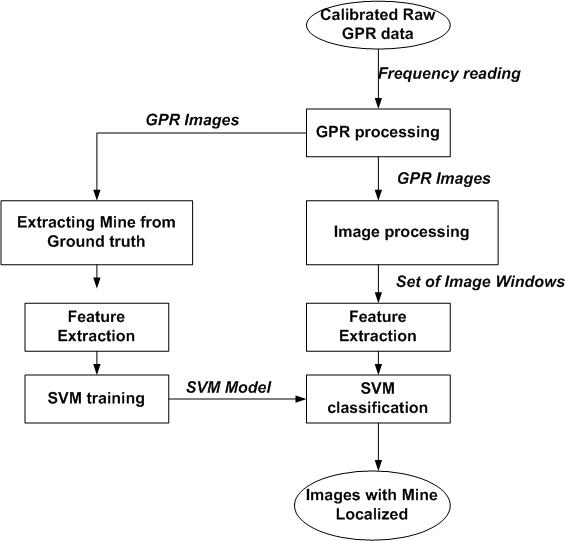
\includegraphics[width=0.45\textwidth]{images/BlockDiagram.jpg}
 \caption{The Block diagram }
\end{figure}



\subsection{GPR processing}

A multistatic ground-penetrating radar (GPR) sys-tem has been developed and used to measure the response of a
number of targets to produce data for the investigation of multi-static inversion algorithms. The system consists of a linear array
of resistive-vee antennas, microwave switches, a vector network
analyzer, and a 3-D positioner, all under computer control. The
array has two transmitters and four receivers which provide eight
bistatic spacings from 12 to 96 cm in 12-cm increments. Buried
targets are scanned with and without surface clutter, which is a
layer of rocks whose spacing is empirically chosen to maximize the
clutter effect. The measured responses are calibrated so that the
direct coupling in the system is removed, and the signal reference
point is located at the antenna drive point. Images are formed us-ing a frequency-domain beamforming algorithm that compensates
for the phase response of the antennas. Images of targets in air
validate the system calibration and the imaging algorithm. Bistatic
and multistatic images for the buried targets are very good, and
they show the effectiveness of the system and processing.

%%% this is from multi experiement paper \ldots.
The multistatic GPR in this paper consists of a linear array
of resistive-vee antennas, a microwave switch matrix, a vector
network analyzer (Agilent 8720D), and a 3-D positioner, all
under computer control (Fig. 1). The resistive-vee antenna ishosen as an array element because it can transmit and receive
short pulses with a negligible amount of clutter, and it has a
low radar cross section, which eliminates most of the multiple
reflections between the antenna and the ground [14]–[16]. In
addition, it is lightweight; therefore, an array of the resistive-vee antennas can be made in a hand-held form. The antenna
was optimized for a bistatic GPR.





he GPR is scanned over a 1.8 × 1.8 m region at a constant
height above the surface of the ground. The scan region is
referenced by x- and y -coordinates, both ranging from −90 to
90 cm in 2-cm increments. Thus, the scan region is discretized into a grid of 91 points by 91 points. The location of the
GPR array in the coordinate system is referenced to the center
point of transmitter T1. Each time the GPR array stops, it
collects data from the eight bistatic spacings by manipulating
switches in an appropriate order. After each switch operation,
the network analyzer sweeps 401 equally spaced frequency
points from 60 MHz to 8.06 GHz. This procedure at each
point takes approximately 6 s. The total scan time is approxi-mately 14 h.

The lowest effective frequency is in the range of 500 MHz–
1.0 GHz because the gain of the antenna falls off quickly in this
frequency range [20]


The data calibrated according to (1) are stored in Matlab
file format. Each Matlab file contains one set of measured and
calibrated data obtained from a single scan of 1.8 × 1.8 m
region. The stored variables are responses from eight bistatic
spacings (401 × 91 × 91 double precision), frequency points at
which the data are measured (401 × 1 double precision), and
x- andy -coordinates of each measurement (91 × 1).


The multistatic GPR is operated on five sets of buried targets.
The target sets are an assortment of metal spheres, a variety
of AT and AP landmines, a Plexiglas box, a plastic pipe,
and empty sand. Table I contains more information about the
landmine and clutter objects. Target depths range from 1 to
58 cm; the depth of a target is measured from the surface of
the sand to the top of the target. The ground medium is damp
compacted sand with a water table below target level.
Each set of targets is scanned with and without surface clutter
according to the following procedure (the buried pipe is done
only with a clean surface). First, the targets are buried, and
the surface of the sand is packed so that the height of the
surface varies less than 2 cm. The sand is then soaked with
water and let stabilize for approximately 2 h. This process is
performed to maintain appropriate moisture level in the sand
and to minimize the disturbance made in the sand when the
targets are buried. The responses of the targets in sand with
a clean surface are obtained as the GPR scans over the sand.
Next, river rocks are randomly scattered over the scan region,
as shown in Fig. 12. The density of the rocks is empirically
chosen to maximize the clutter effect. In both the clean-surface
and cluttered-surface scans, the antenna array is elevated by
10 cm, which is measured from the surface of the sand to the
bottom of the antenna array.

 \begin{figure}
\centering
\label{fig:minloc}
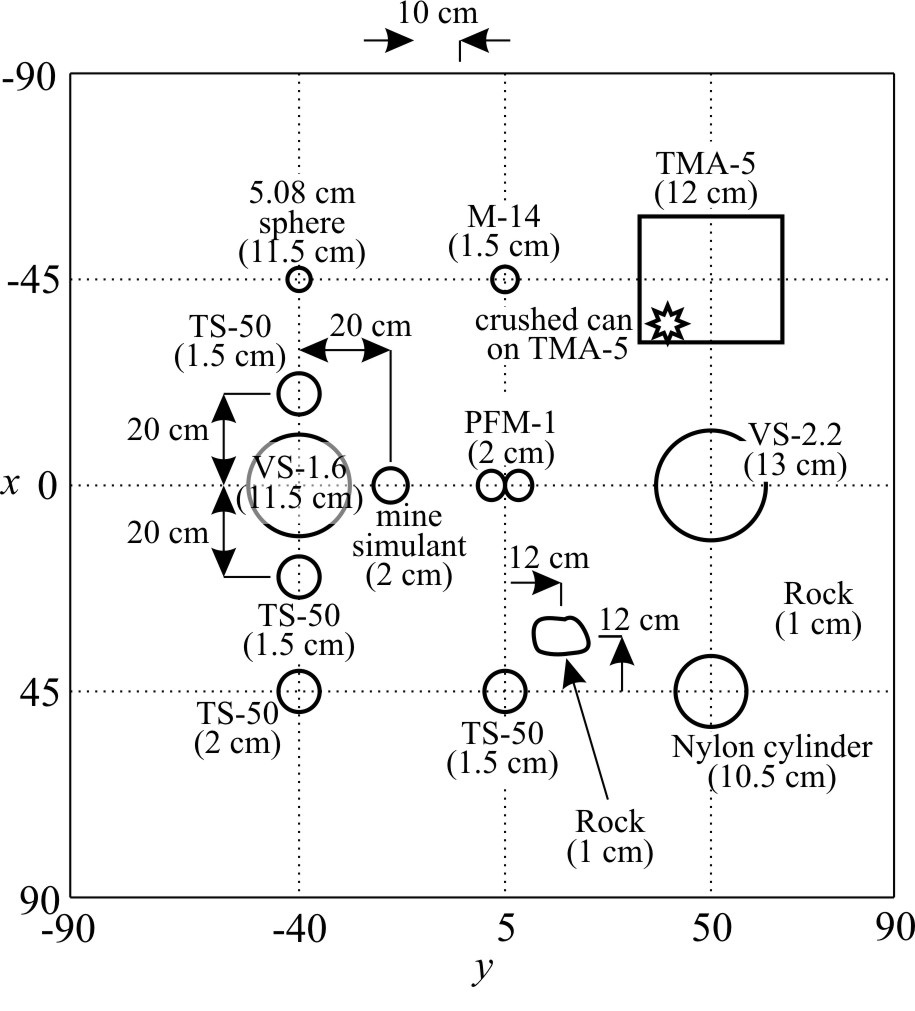
\includegraphics[width=0.45\textwidth]{images/MineLocations.jpg}
 \caption{Mine Locations}
\end{figure}

 \begin{figure}
\centering
\label{fig:mineshapes}
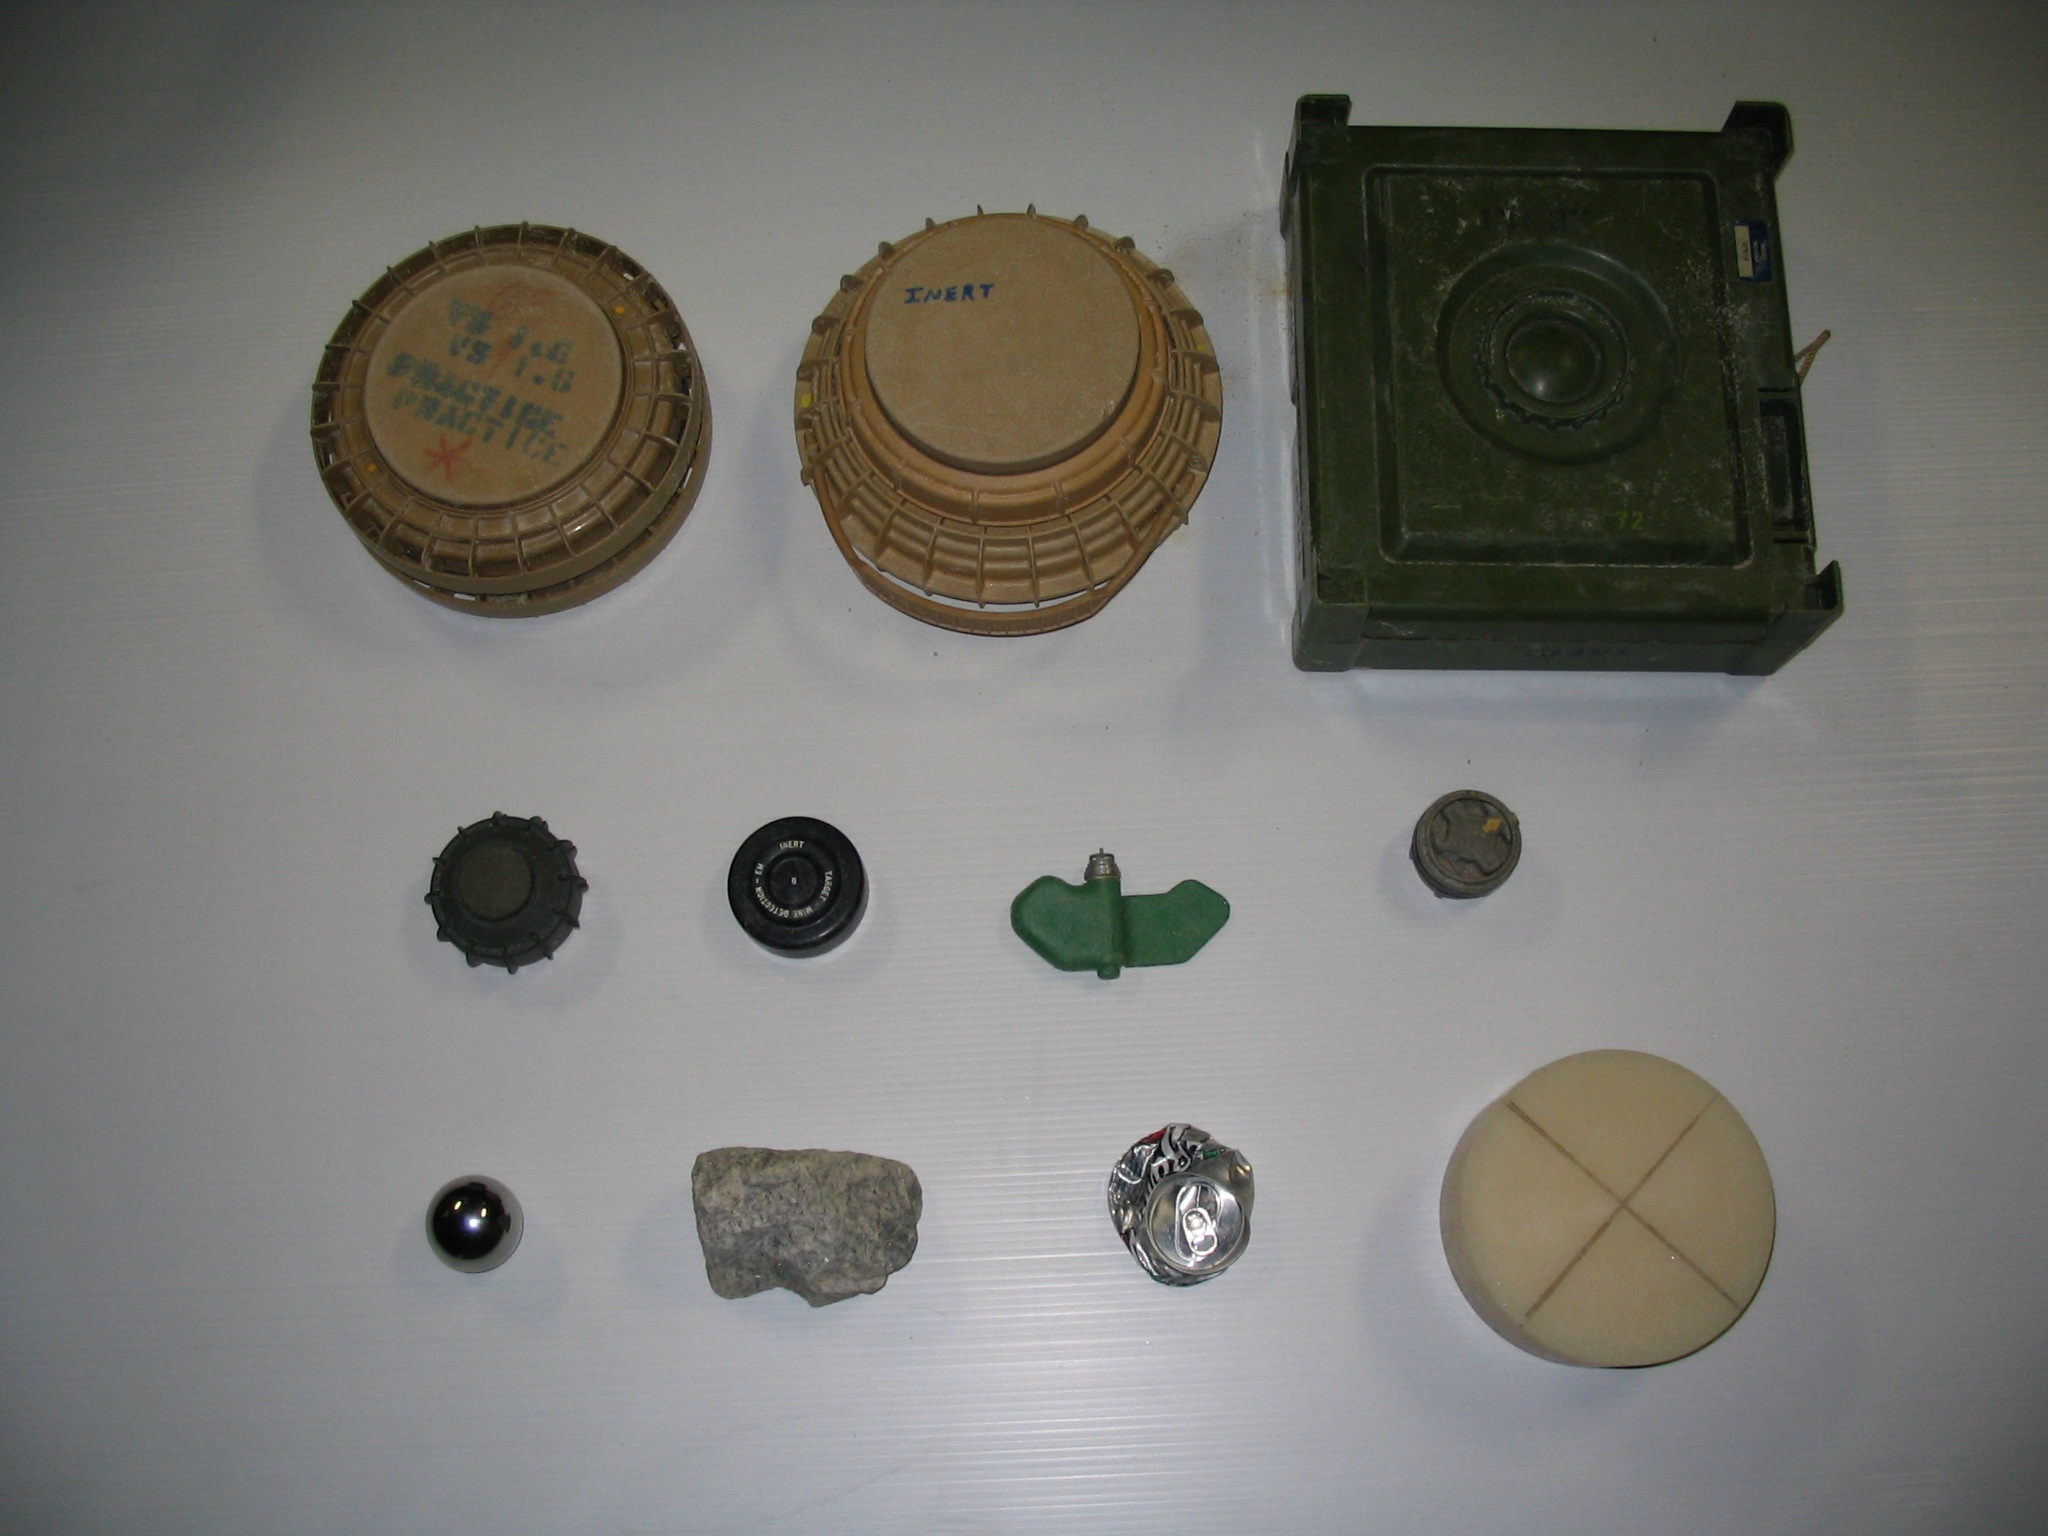
\includegraphics[width=0.45\textwidth]{images/MineShapes.jpg}
 \caption{ Sample of mines  }
\end{figure}


More plain text
\subsection{Image processing}


Gradient Features
To extract gradient features [3], the gradient operator is first applied to the gray-scale image of the digit to give two gradient components: strength |g(x,y)| and direction  at each point (x,y) of the image f. This is done by applying Sobel operator [20] on the image to extract vertical and horizontal gradient components,
 ,	(2)
 ,	(3)
where f(x,y) is the intensity of image f at point (x,y), gx(x,y) is the gradient component at x-direction at location (x,y), and gy(x,y) is the gradient component at y-direction at location (x,y).
Then the gradient strength and direction is extracted using equations (4) and (5), respectively,
 		(4)
 			(5)
The gradient vector g(x,y) (expressed as strength strength |g(x,y)| and direction  ) at each point (x,y) of the image is then decomposed into the 8 Freeman [20] directions shown in Fig. 2. The gradient vector is decomposed into the 8 Freeman directions by projecting the vector into the nearest two Freeman directions as shown in Fig. 3.
The gradient features are composed of 8 layers; each corresponding to one of the Freeman directions. Each layer is the projection of the gradient vectors of the image into the corresponding Freeman direction.
A Gaussian mask h(x,y) is then applied to each layer,
 ,		(6)
and then the layers are uniformly sampled to give 5×5 measurements. The parameter σ is related to the sampling interval t via the empirical relation  [3]. This means that the gradient features are composed of 8×5×5 = 200 elements. The gradient feature extraction technique is very powerful as shown in [3] and as will be shown in the results section (section 5) of this paper.
4.2 Kirsch Features
The Kirsch features [3] are extracted by decomposing the image into 4 layers corresponding to 4 edge orientations: horizontal (gh), vertical (gv) , right diagonal (grd), and left diagonal (gld). These layers are extracted by applying Kirsch masks on the image,
 ,		(7)
 ,		(8)
 ,	(9)
 ,	(10)
where * denotes 2D convolution operation [20], kh1 and kh2 are Kirsch masks responsible for extracting horizontal edges, kv1 and kv2 for horizontal edges, krd1 and krd2 for right diagonal edges, and kld1 and kld2 for left diagonal edges. Figure 4 shows all Kirsch masks.
gh1
5	5	5
-3	0	-3
-3	-3	-3
	gh2
-3	-3	-3
-3	0	-3
5	5	5
	gv1
5	-3	-3
5	0	-3
-3	-3	-3
	gv2
-3	-3	5
-3	0	5
-3	-3	5

grd1
-3	-3	-3
5	0	-3
5	5	-3
	grd2
-3	5	5
-3	0	5
-3	-3	-3
	gld1
-3	-3	-3
-3	0	5
-3	5	5
	gld2
5	5	-3
5	0	-3
-3	-3	-3

Figure 4. Kirsch  Masks

A Gaussian mask is then applied to all the 4 layers and 5×5 measurements are extracted from each of them in the same manner done with gradient features (section 4.1). This means that Kirsch features are composed of 4×5×5=100 elements.
4.3 Local Chain Code Features
To extract the local chain code features [21], the contour of the digit is first followed by any contour following algorithm, and then each contour point of the image is marked with the corresponding Freeman direction. The image is then decomposed into 8 layers; each layer contains only contour points that belong to the corresponding Freeman direction. Each of the 8 layers is then uniformly partitioned into 5×5 zones. Each zone is averaged leading to a feature vector of 200 elements.


4.4 Wavelet Features
Wavelet transform [20] extracts the essential information contained in a signal or image. This may help in reducing the dimensionality of the problem which leads to faster classification. Also it might reduce the noise and the non-essential information that may confuse the classifier leading to better classification performance. Wavelet transform could be applied on the image directly or could be applied on the gradient decomposition of the image [22]. In our study, we applied the former method. The image is first resized to be 64×64 and then the image is composed into 3 resolution levels. The 3rd level approximation of the image (which is a 8×8 image) is then used as features. This means that wavelet features are composed of 64 elements.
4.5 Concatenation of low dimensional features
Here we concatenate 6 families of low dimensional features to form one feature vector. While each of these low dimensional features is not very effective, their concatenation proved to be a powerful feature vector. Each of the 6 low dimensional feature families is going to be discussed in the following subsections.
4.5.1 Raw Image Zoning
In this technique, the image is uniformly partitioned into 5×5 zones [23]. The average of each zone is calculated leading to a feature vector of 25 elements.

4.5.2 Vertical and Horizontal Projections
In this technique, the horizontal and vertical histograms of the image are calculated leading to a feature vector of 40 elements [23] (Remember that we are working on the 20×20 window that confines the digit not all 28×28 pixels of the MADBase digits).


4.5.3 Vertical and Horizontal Cross Counts
The image is first binarized, and then the vertical and horizontal cross counts are calculated leading to a feature vector of 40 elements.
4.5.4 Centroidal Distances
In this technique [11, 24], the digit image is partitioned into 16 sectors around the digit center of gravity (the centroid) as shown in Figure 5. Then the centroid of each sector are calculated. The distances between the whole digit centroid and sectors centroids are calculated and normalized by dividing them by the digit bounding box diameter. This forms a 16-element feature vector.
4.5.5 Directional Features
The directional features are formed as follows [11, 25]. Each background pixel is labeled by a 4-element vector. For each background pixel we walk upward; if a foreground pixel is found, the first element of the 4-element vector is set to ‘1’ otherwise set to ‘0’. Then we walk to the right; if a foreground pixel is found, the second elements is set to ‘1’ otherwise set to ‘0’; and so on till we finish the 4 principal directions. Then for each combination of 0’s and 1’s in the 4-element vector, we give a different label. Hence, we have 16 different labels. Now each of foreground pixels has one label of the 16 labels. The final feature vector is the histogram of such labels giving rise to a 16 element feature vector.
4.5.6 Length-Normalized Contour
In this technique [11], the horizontal and vertical coordinates of the boundary pixels of the digit are used as features. First, the boundary of the digit is extracted using a contour following algorithm; then, each boundary point is stored by its horizontal and vertical coordinates. Horizontal locations are magnitude-normalized by dividing them by the width of the digit bounding box. Vertical locations are also magnitude-normalized by dividing them by the height of the bounding box. Then both horizontal and vertical locations are partitioned into 10 portions and the average of each portion is calculated leading to a feature vector of length 20.
Feeding the classifier with the concatenation of different features without any preprocessing step would lead to very bad results because features of large magnitudes will dominate. Hence, we applied mean and variance normalization [14] to all the low-dimensional features discussed in this section before concatenating them into a feature vector of length 156.
4.6 Local Directional Features
Local directional features extraction is a novel technique that we present in this paper. It is a natural extension of the directional features presented in section 4.5.5. Like directional features, each background pixel is labeled by a 4-element vector which leads to 16 different labels. However not all labels are used. Only 9 labels corresponding to 9 situations are considered: (1) closed from all directions (i.e. black pixel can be reached when moving in all the principal 4 directions), (2) open up (i.e. black pixel can be reached when moving in the principal 4 directions except when moving upward), (3) open down, (4) open right, (5) open left, (6) open up and right, (7) open up and left, (8) open down and right, and (9) open down and left.
The image is then decomposed into 9 layers; each layer corresponds to one of the 9 labels. Pixel (x,y) in layer #n is illuminated only if pixel (x,y) in the image has been given the label #n. A Gaussian mask is then applied to all the 9 layers and 5×5 measurements are extracted from each of them in the same manner done with gradient features (section 4.1). This means that local directional features are composed of 225 elements




\subsection {Classification}

%The input of the feature extraction method is four different feature vector based on orientation used. A classifier is used for each orientation which means that the feature vector for each classifier consist of  $9\timesn$ concavity map. To simplify the classification we use simple one versus one (OVO) Support Vector Machine (SVM) using linear kernel classifier. Since the SVM is a binary classifier we used One versus one configuration for the classifiers which requires
The output of the feature extraction stage is four different feature vectors for the four different orientations used. A classifier is used for each orientation. To simplify the classification we use simple one versus one (OVO) Support Vector Machine (SVM) with linear kernel classifier. Since the SVM is a binary classifier, the one versus one classification requires $\frac{n(n-1)}{2}$ classifiers for $n$ classes. The final decision of the classification in a one versus one classifier can be obtained using simple majority voting. Unfortunately, this method does not generate the confidence measure for each class needed in the classifier fusion step. Various methods can be used to generate such probability or confidence measure from pairwise classifiers. One of the popular methods is introduced in \cite{pairwise22} where $p_i$ probability of sample $x$ to belong to class $i$  is computed using the following equation :

%The output of the feature extraction stage is four different feature vectors for the four different orientations used. A classifier is used for each orientation. To simplify the classification we use simple one versus one (OVO) Support Vector Machine (SVM) with linear kernel classifier. Since the SVM is a binary classifier, the one versus one classification requires $\frac{n(n-1)}{2}$ classifiers for $n$ classes. The final decision of the classification in a one versus one classifier can be obtained using simple  majority voting. Unfortunately, this method does not generate a confidence measure for each class which is needed in the classifier fusion step. Various methods can be used to generate such probability or confidence measure from pairwise classifiers. One of the popular methods is introduced in \cite{pairwise22} where $p_i$ probability of sample $x$ to belong to class $i$  is computed using the following equation :
%
% The final decision of the classification can be extraction using various method. One of the simple methods is majority voting.  Unfortunately, this method does not generate a confidence measure for each class which we need in the classifier fusion step. Various methods were used to generate such  probability or  confidence measure from pairwise classifiers. One of the popular methods used is introduced in \cite{pairwise22} where
%  \[
% p_i=\frac{1}{r_{ij}k-1}
% \]
\[
P_i(x)  = \frac{1}{{\sum\limits_{j = 1,j \ne i}^K {\frac{1}{{r_{ij}(x) }} - (K - 2)} }}
\]

where $r_{ij}(x)$   is the probability of the tested pattern $x$ to be of class $i$, where the used classifier is the one responsible for separating class $i$ from class $j$  and $k$ is the number of classes.

\subsubsection{Fusion Methods}
Fusion methods can be divided into three main categories: label based, rank based, and soft margin or fuzzy based methods. The label based method are usually based on the final label of base classifiers like the majority voting fusion. The rank based method uses the decision values of base classifiers to rank using various fixed rules to get the final decision for the system. The soft margin and fuzzy based methods use the output decision values of the base classifiers as a pattern recognition problem and try to detect the correct pattern. Methods like Bayes and neural network fusion are considered the most widely used fusion methods based on this type  \cite{Farah2005,Ruta2000,Denoeux2000}.
%(For example : Sum, Max, Min, Mean and Borda Count)
%Fusion methods can be divided into three main categories Label based, Rank based and soft margin or fuzzy based methods. The label based method are usually based on the final label of base classifiers like the majority voting fusion. The rank based method uses the decision values of base classifier to rank uses various fixed rule to get the final decision value for the system. The soft margin and fuzzy based methods tries to use the output decision values  of the base classifier as a pattern recognition problem and tries to try to detect the correct pattern. Methods like Bayes and neural network fusion is considered the most fusion method based on this type. .



%The four base classifiers generate a set of normalized probability for each class $P_i(x)$ for a given input sample $x$. These probabilities are as input the fusion methods.

The four base classifier generate the posterior probabilities $P_{ij}(x), i = 1\dots c; j = 1\dots k$ for $c$ classifiers and $k$ classes is computed for test sample $x$. A fusion method will  combine them to a new set of probability  $q_j(x)$ which can be used for the final classification. Let $q_j(x)$ be computed by $q_j(x)=rule_i\left(P_{ij}(x)\right)$. The final classification is made by $\phi(x)=\max\limits_j(q_j(x))$. The rules we used to compute $q_j(x)$ are Majority vote, Maximum, Minimum, Mean, Median, Sum, Weighted Sum, Product and Borda Count. %summarized below:

\section{Experiments}
\section {Results}

%develop new features based on structural information.
\bibliographystyle{IEEEtran}
\bibliography{library,Landmine}
\end{document}
